% Setting the Preamble
\documentclass[12pt]{article}
%\usepackage{extsizes}
\usepackage{booktabs}
\usepackage{rotating}
\usepackage{mathtools}
\usepackage{amssymb}
\usepackage[american]{babel}
\usepackage{float}
\usepackage{array} % for defining a new column type
\usepackage{varwidth} %for the varwidth minipage environment
\usepackage{acronym}
\usepackage{fullpage} %for adjusting margins
\usepackage{ragged2e} %for justification of text
\usepackage{amsmath}
\usepackage{multicol}
\usepackage{dcolumn}
\usepackage{threeparttable}
\usepackage{lscape}
\usepackage{longtable}
\usepackage{caption}
\usepackage{graphicx}
\usepackage{subcaption}
%\usepackage[total={5.5in, 8.5in}]{geometry}
\usepackage[bottom]{footmisc}
\usepackage{setspace}
%\doublespace
\usepackage[normalem]{ulem}
\usepackage{color,soul} %Use to highlight/colour text
\usepackage{xcolor} %Use to highlight/colour text
\usepackage{geometry}
\geometry{verbose,tmargin=3cm,bmargin=3cm,lmargin=2cm,rmargin=2cm}
\setcounter{secnumdepth}{2}
\setcounter{tocdepth}{2}
\usepackage{prettyref}
\usepackage{amsmath}
\usepackage{amsthm}
\usepackage{amssymb}
\usepackage{graphicx}
\usepackage{setspace}
\usepackage{esint}
\setstretch{1}
\usepackage[unicode=true]
 {hyperref}
%\usepackage{xcolor}
\hypersetup{
    colorlinks,
    linkcolor={blue!70!black},
    citecolor={blue!70!black},
    urlcolor={black!70!black}
}
%\usepackage[style=Matlab-editor]{mcode}
\usepackage{matlab-prettifier}
\graphicspath{{images/}}
%%%%%%%%%%%%%%%%%%%%%%%%%%%%%% Textclass specific LaTeX commands.
 \theoremstyle{definition}
 \newtheorem*{defn*}{\protect\definitionname}
\theoremstyle{plain}
\newtheorem{thm}{\protect\theoremname}[section]
  \theoremstyle{plain}
  \newtheorem{lem}[thm]{\protect\lemmaname}
  \theoremstyle{remark}
  \newtheorem{claim}[thm]{\protect\claimname}
  \theoremstyle{plain}
  \newtheorem{prop}[thm]{\protect\propositionname}

\makeatother

\usepackage{babel}
  \providecommand{\claimname}{Claim}
  \providecommand{\definitionname}{Definition}
  \providecommand{\lemmaname}{Lemma}
  \providecommand{\propositionname}{Proposition}
\providecommand{\theoremname}{Theorem}



\usepackage{listings}
\usepackage{color} %red, green, blue, yellow, cyan, magenta, black, white
\definecolor{mygreen}{RGB}{28,172,0} % color values Red, Green, Blue
\definecolor{mylilas}{RGB}{170,55,241}

\DeclareMathOperator*{\argmax}{arg\,max}
\DeclareMathOperator*{\argmin}{arg\,min}

\usepackage{physics}
\usepackage{natbib}
\usepackage{titling}
\usepackage{blindtext}
\renewcommand{\thesection}{\arabic{section}}
\setcounter{secnumdepth}{3}
\setcounter{tocdepth}{3}
%\newtheorem{prop}{Proposition}
\usepackage{epigraph}
\renewcommand\textflush{flushright}

    \usepackage{etoolbox}
    \makeatletter
    \newlength\epitextskip
    \pretocmd{\@epitext}{\em}{}{}
    \apptocmd{\@epitext}{\em}{}{}
    \patchcmd{\epigraph}{\@epitext{#1}\\}{\@epitext{#1}\\[\epitextskip]}{}{}
    \makeatother

    \setlength\epigraphrule{0pt}
    \setlength\epitextskip{2ex}
    \setlength\epigraphwidth{.9\textwidth}
%%%%%%%%%%%%%%%%%%%%%%%%%%%%%%%%%%%%%%%%%%%%%%%%%%%%%%%%%%%%%%%%%%%%%%%%%%%%%%%%%%%%%%%%%%%%%%%%%%%%%%%%%%%%%%%%%%%%
\title{\textbf{(Dis)Inflation Targeting}}
\date{}
\author{\textit{Mridula Duggal}\thanks{Universitat Aut\`onoma de Barcelona (UAB) and Barcelona Graduate School of Economics (BGSE). Email: mriduduggal@gmail.com.} \mbox{ and }\textit{Luis Eduardo Rojas}\thanks{Markets, Organisation and Votes in Economics(MOVE), Universitat Aut\`onoma de Barcelona (UAB), Barcelona Graduate School of Economics (BGSE). Email:luis.rojas@MOVEbarcelona.eu}}
\onehalfspacing
\begin{document}
\begin{titlepage}
\clearpage\maketitle
\thispagestyle{empty}
    \justify
    \begin{abstract}
    \textcolor{red}{TO BE COMPLETED}
    \end{abstract}
\end{titlepage}
%\tableofcontents
\newpage
\section{Introduction}
\textcolor{red}{TO BE COMPLETED}

\section{Motivation}
\justify
As Figure \ref{fig:figure1} and Figure \ref{fig: figure3} portray, Colombia and Brazil are examples of the process of disinflation that economies experience when adopting Inflation Targeting. Both countries adopted inflation targeting when they were experiencing episodes of high inflation post the oil crisis in the late 1980s and the East Asian Financial crisis in 1997. 

\begin{figure}[H]
\centering 
\caption{Inflation Target, Actual Inflation and Inflation Expectations: Colombia} 
\label{fig:figure1}
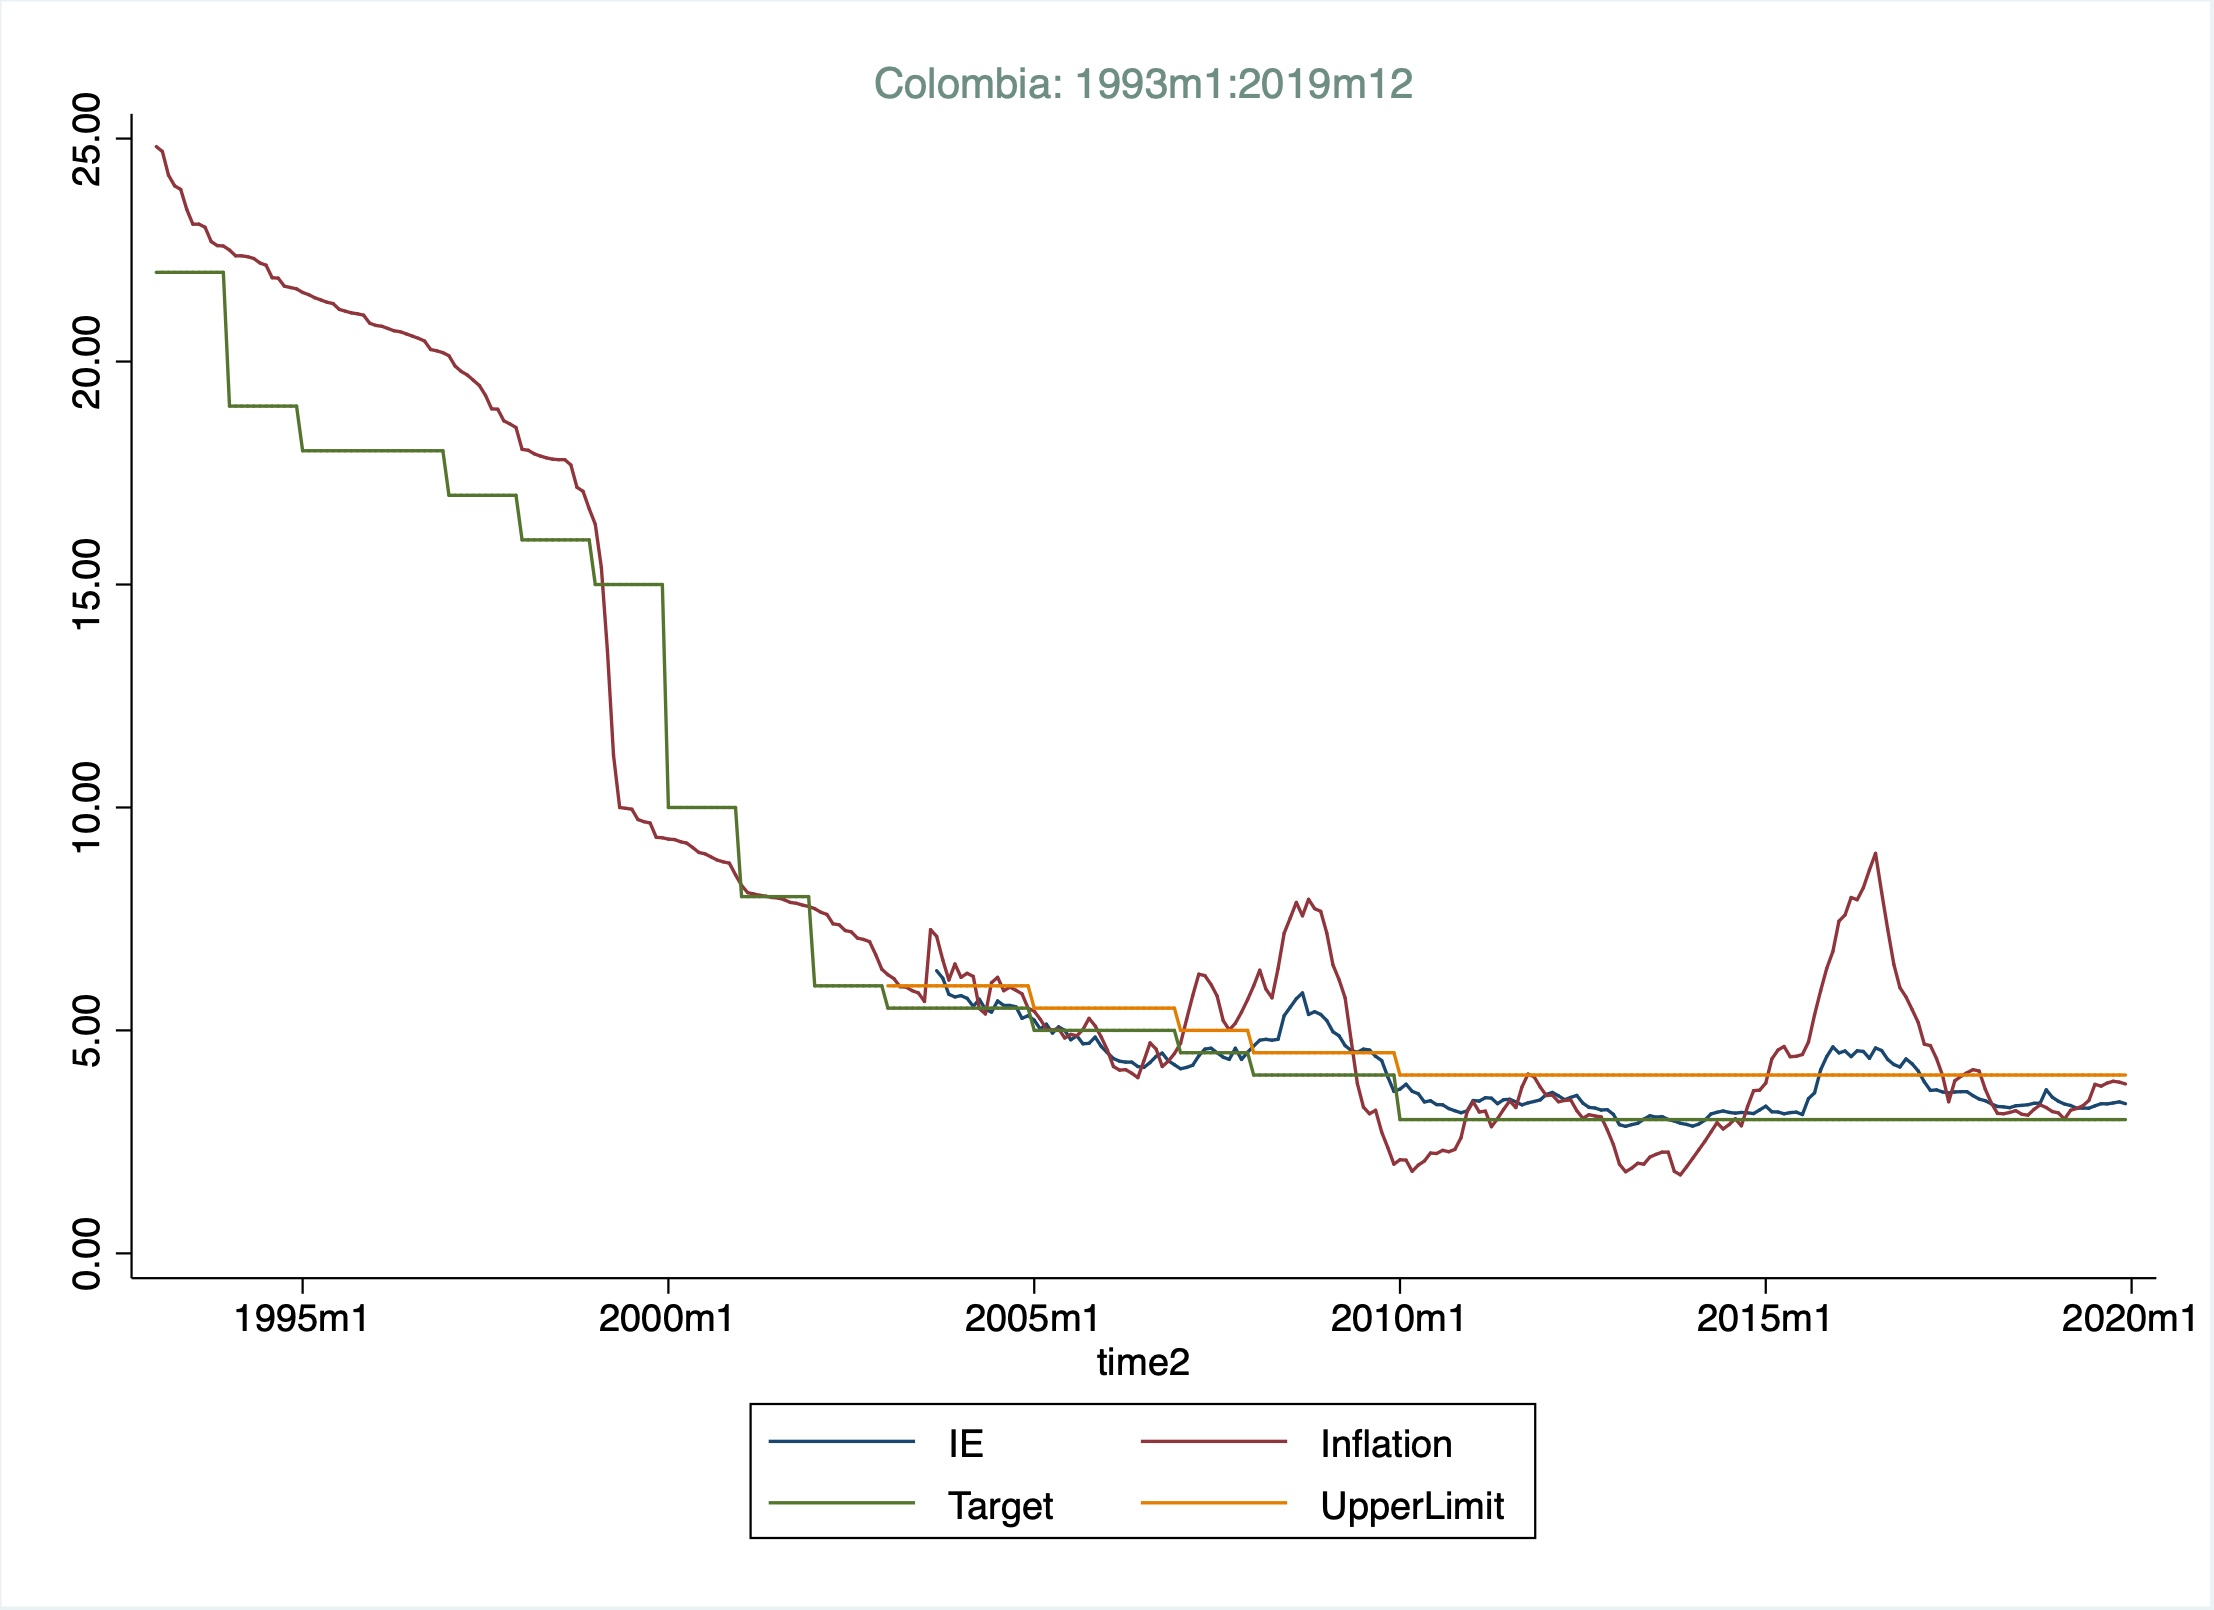
\includegraphics[width=12cm, height=7cm]{Colombia}
\end{figure}

%\begin{figure}[H]
%\centering 
%\caption{Long Run Trend and Central Bank Targets, Source: \cite{echavarria2011target}} 
%\label{fig:figure2}
%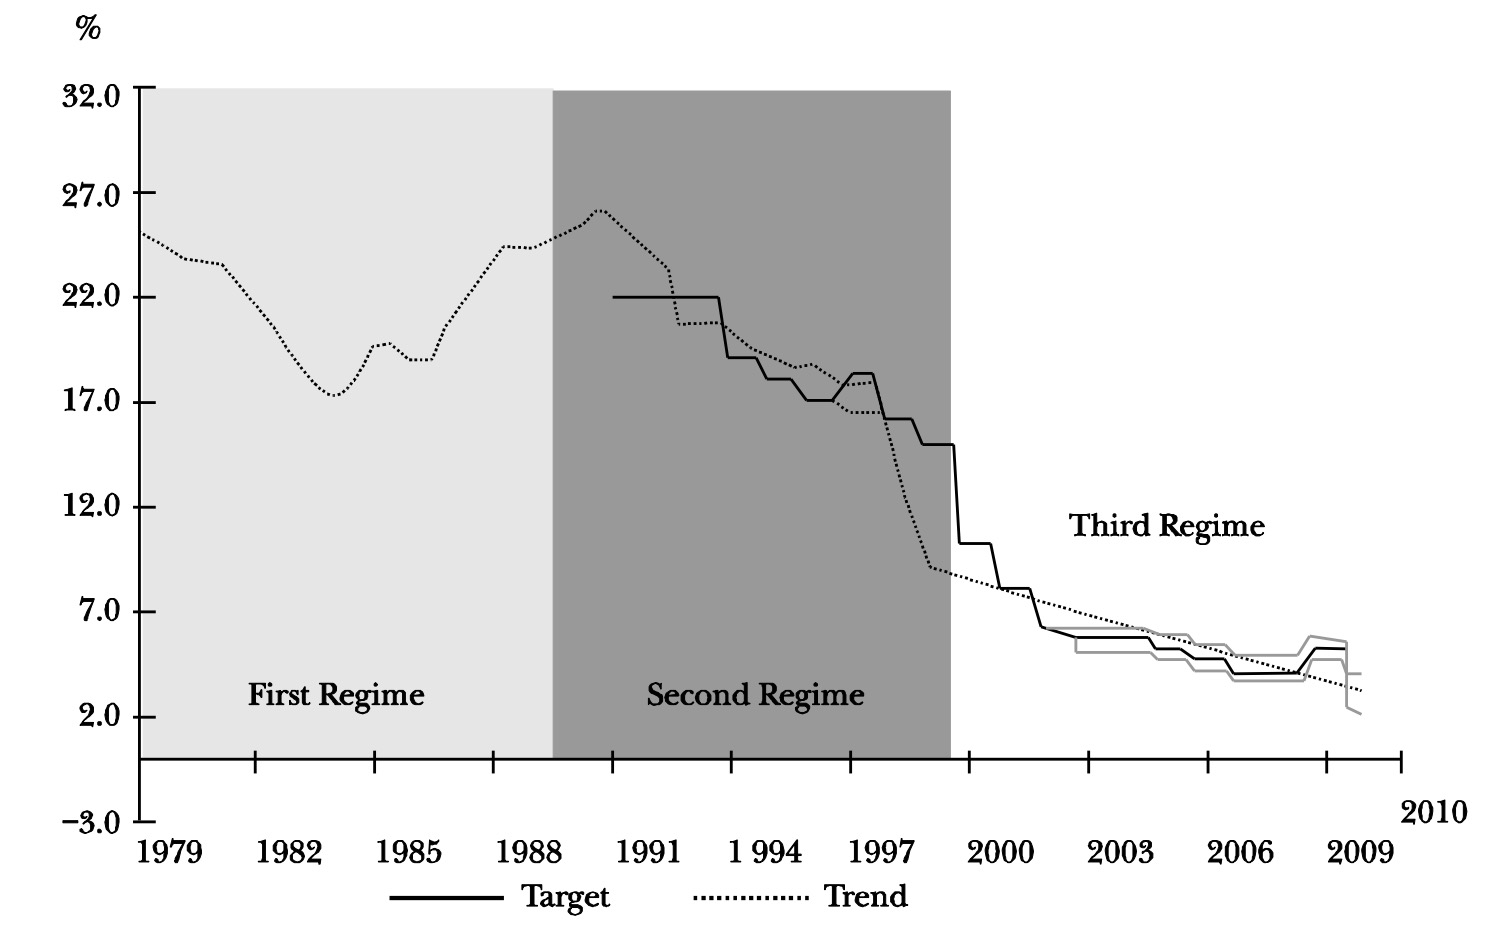
\includegraphics[width=12cm, height=7cm]{Rojas}
%\end{figure}


\begin{figure}[H]
\centering 
\caption{Inflation Target, Actual Inflation and Inflation Expectations: Brazil} 
\label{fig: figure3}
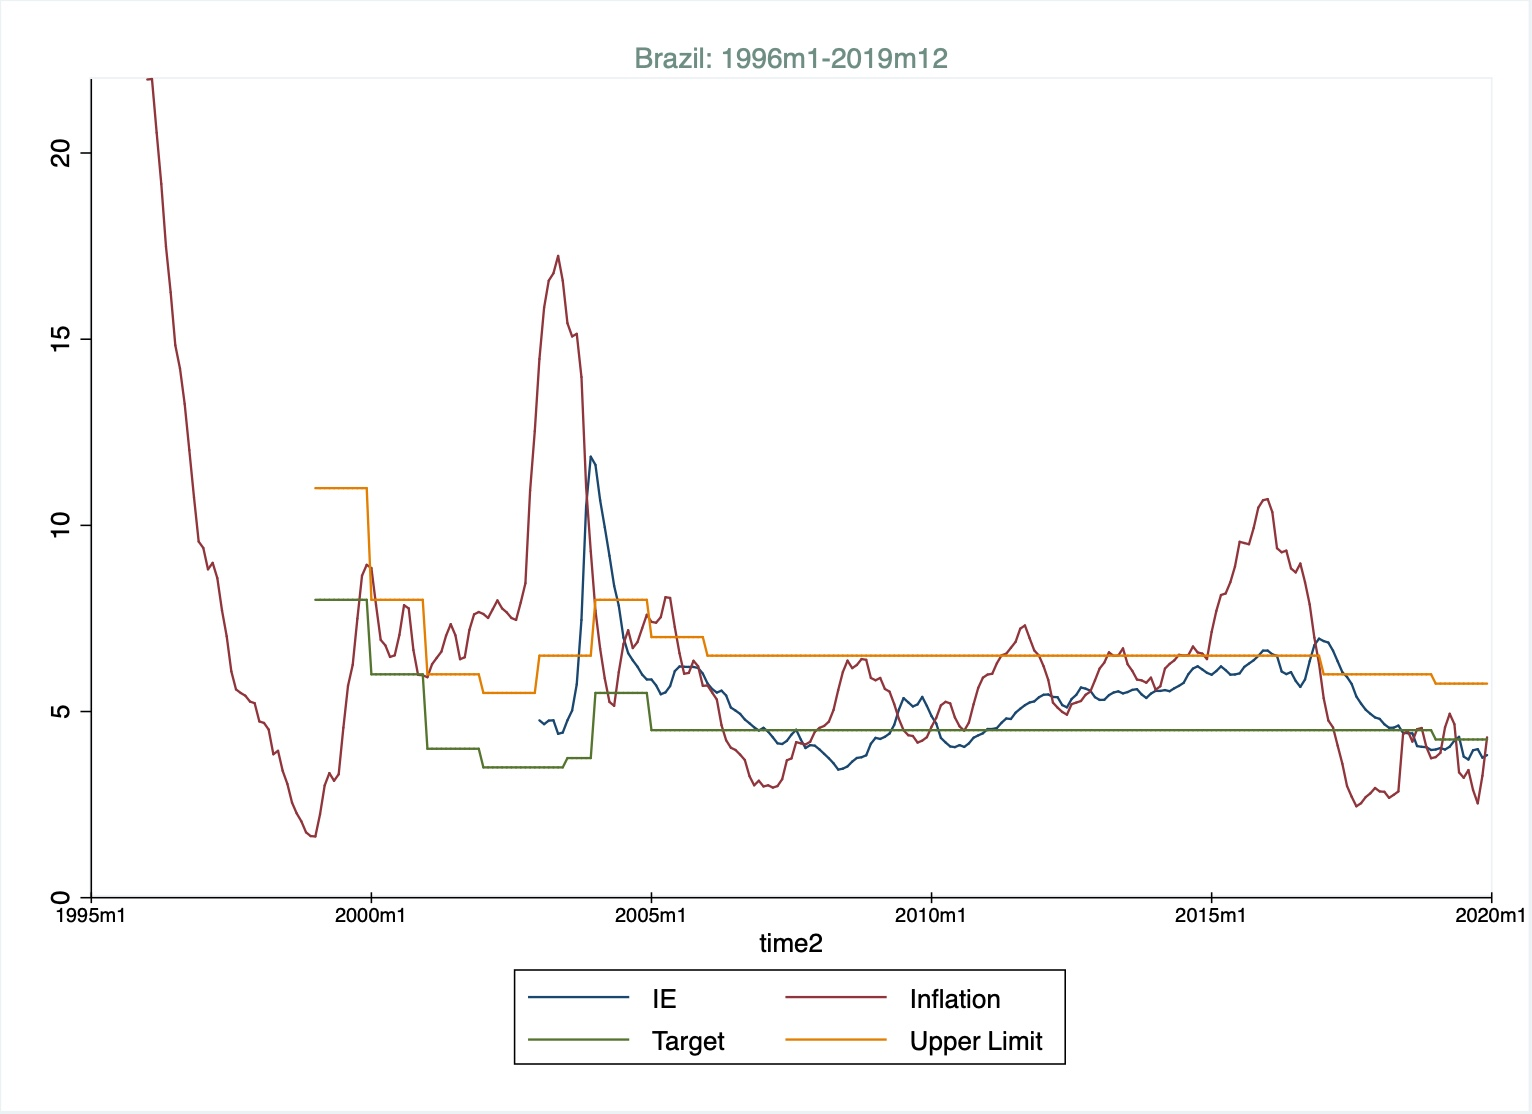
\includegraphics[width=12cm, height=7cm]{Brazil}
\end{figure}

\section{Model}
\justify
The preferences of the government are given by 
\[
z_{t}=\frac{a}{2}\left(\pi_{t}\right)^{2}-b_{t}(\pi_{t}-\pi_{t}^{e})
\]
\justify
and expectations formation are as follows:
\begin{itemize}
\item If $\pi_{t}\leq\pi_{t}^{e}$ then $\pi_{t+1}^{e}=\max\left\{ \gamma\pi_{t},\pi_{t+1}^{\ast}\right\} $,
where $\pi_{t+1}^{\ast}$ is the announced inflation target at $t+1$.
\item For $\gamma=0$ we have the Barro-Gordon case.
\item If $\pi_{t}>\pi_{t}^{e}$ then $\pi_{t+1}^{e}=\frac{\bar{b}}{a}$ the discretionary outcome ($\bar{b}$ is the expected $b_{t+1})$
\end{itemize}

\subsection*{Case 1: Disinflation follow the threshold $\pi_{t+1}^{\ast}=\gamma\pi_{t}$}
\justify
In this case the discounted value for the government is 
\[
V_{0}=\sum_{t=0}^{\infty}\beta^{t}\left[\frac{a}{2}\left(\gamma^{t}\frac{b}{a}\right)^{2}\right]=\sum_{t=0}^{\infty}\beta^{t}\left[\frac{b^{2}}{2a}\gamma^{2t}\right]=\frac{b^{2}}{2a}\frac{1}{1-\beta\gamma^{2}}
\]
\justify
and starting form any arbitrary $t=s$ we have 
\[
V_{s}=\sum_{t=0}^{\infty}\beta^{s}\left[\frac{a}{2}\left(\gamma^{s+t}\frac{b}{a}\right)^{2}\right]=\sum_{t=0}^{\infty}\beta^{s}\left[\frac{b^{2}}{2a}\gamma^{2(s+t)}\right]=\frac{b^{2}}{2a}\gamma^{2(s)}\frac{1}{1-\beta\gamma^{2}}=\gamma^{2(s)}V_{0}
\]

\justify
Is it worthy to deviate? the value in case the government deviates
is 
\begin{align*}
V_{d,s} & =\frac{a}{2}\left(\frac{b}{a}\right)^{2}-b_{t}(\frac{b}{a}-\gamma^{s}\frac{b}{a})+\beta V_{0}\\
 & =\frac{b^{2}}{2a}-\frac{b^{2}}{a}(1-\gamma^{s})+\beta V_{0}
\end{align*}
\justify
then it is optimal to deviate if 
\begin{align*}
\frac{b^{2}}{2a}-\frac{b^{2}}{a}(1-\gamma^{s})+\beta V_{0} & \leq\gamma^{2(s)}V_{0}\\
\frac{b^{2}}{2a}-\frac{b^{2}}{a}(1-\gamma^{s}) & \leq\left(\gamma^{2(s)}-\beta\right)V_{0}\\
\frac{\frac{b^{2}}{a}\left(\gamma^{s}-\frac{1}{2}\right)}{\left(\beta-\gamma^{2(s)}\right)} & \leq V_{0}\\
\frac{\left(2\gamma^{s}-1\right)}{\left(\beta-\gamma^{2(s)}\right)} & \leq\frac{1}{1-\beta\gamma^{2}}
\end{align*}
\justify
with $\gamma=0$ we recover the Barro-Gordon case where zero inflation
is not sustainable as 
\[
\frac{\left(-1\right)}{\left(\beta\right)}\leq1
\]
\justify
holds.
\justify
When $s=\infty$ we have 

\begin{align*}
\frac{b^{2}}{2a}-\frac{b^{2}}{a}+\beta V_{0} & \leq0\\
V_{0} & \leq\frac{1}{\beta}\frac{b^{2}}{2a}\\
\frac{b^{2}}{2a}\frac{1}{1-\beta\gamma^{2}} & \leq\frac{1}{\beta}\frac{b^{2}}{2a}\\
\gamma^{2} & \leq\frac{1}{\beta}-1
\end{align*}
\justify
this sets a lower bound on $\gamma$. So to have no incentives to
deviate at the limit it has to be that 
\begin{align*}
\gamma^{2} & \geq\frac{1}{\beta}-1\\
\gamma & \geq\left(\frac{1}{\beta}-1\right)^{1/2}
\end{align*}
\justify
Going back to the previous condition
\begin{align*}
\frac{b^{2}}{2a}-\frac{b^{2}}{a}(1-\gamma^{s}) & \leq\left(\gamma^{2(s)}-\beta\right)V_{0}\\
-\frac{1}{2}\frac{b^{2}}{a} & \leq\left(\gamma^{2(s)}-\beta\right)V_{0}-\frac{b^{2}}{a}\gamma^{s}\\
-\frac{1}{2} & \leq\left(\gamma^{2(s)}-\beta\right)\frac{1}{2}\frac{1}{1-\beta\gamma^{2}}-\gamma^{s}
\end{align*}
\justify
is there a $\gamma$ for which this condition is not satisfied for
any $s$? In this case we would be able to implement the efficient
allocation. 
\justify
Yes! There are values of $\gamma$ for which the condition above is
never satisifed for any $s$ and consequently $\pi=0$ can be implemented
in the long run. See the numerical solutions in the matlab file test.m

\justify
The minimum level of inflation achievable with $\gamma=0$ is given
by 
\[
\pi^{BG}=\frac{1-\beta}{1+\beta}\frac{b}{a}
\]
and the value is then given by 
\[
V^{BG}=\frac{1}{2}\frac{b^{2}}{a}\frac{1-\beta}{\left(1+\beta\right)^{2}}
\]
\justify
so the Barro Gordon porvides higher welfare ex-ante than our case
with $\gamma>0$. Down the road for $s>1$ then the welfare in our
case is greater and at the limit $s\rightarrow\infty$ the loss in
our case is zero.
\justify
So the plan is not dinamically consistent without the constraint of
$\gamma$. 

\newpage
\subsection{Optimal Policy}

\textcolor{red}{We are asusming that the solution to the problem is time consistent by assuming that $\gamma_{t}$ is expgenous and deterministic and the policy function that solves the optimality conditions does not depend on the period which the central bank optimises. NEED TO CHECK!} 

\justify
Expectation Formation
\begin{equation}
\pi^{e}_{t+1} = \gamma_{t}\pi_{t} + (1-\gamma_{t})\pi^{a}_{t+1} 
\end{equation}

\justify
IS Curve
\begin{equation}
y_{t} =b_{t}(\pi_{t}-\pi^{e}_{t}) \\
\end{equation}

\justify
Updating Equation
\begin{equation}
\gamma_{t+1} =(1-\theta)\gamma_{t} + \theta(\pi_{t+1} - \pi^{a}_{t+1}) 
\end{equation}

\justify 
Preferences of the Central Bank are given by, 

\begin{equation}
z_{t} = \frac{a}{2} (\pi_{t})^{2} - b_{t}(\pi_{t}-\pi^{e}_{t}) = \frac{a}{2} (\pi_{t})^{2} - y_{t} 
\end{equation}

\justify 
Central bank is optimising the inflation by announcing the target, given inflation expectations. It is an infinite hoirzon problem and they will optimise every period. 

\justify 
The central bank problem is stated as follows, 

\begin{equation}
\min_{\{\pi_{t}, \pi^{a}_{t+1}, \pi^{e}_{t+1}, \gamma_{t+1}\}^{\infty}_{t=0}} E_{0} \sum^{\infty}_{t=0} \beta^{t}\Big[\frac{a}{2} (\pi_{t})^{2} - b_{t}(\pi_{t}-\pi^{e}_{t})\Big]
\end{equation}
\justify
subject to (1), (2) and (3) and a given $\gamma_{0}$. 

\justify
The Lagrangian is given by, 

\begin{equation}
\begin{split}
E_{0} \sum^{\infty}_{t=0} \beta^{t}\Big[\frac{a}{2} (\pi_{t})^{2} - b_{t}(\pi_{t}-\pi^{e}_{t})] \\
+ \lambda_{1t}[\pi^{e}_{t+1} - \gamma_{t}\pi_{t} - (1-\gamma_{t})\pi^{a}_{t+1}] \\
+ \lambda_{2t}[\gamma_{t+1} - (1-\theta)\gamma_{t} - \theta(\pi_{t+1} - \pi^{a}_{t+1}) \Big]
\end{split}
\end{equation}

\justify 
The first order conditions at every $t \geq 0$ are, 

\begin{align}
&{\pi_{t}}: \mbox{  }a\pi_{t}- b_{t} - \lambda_{1t}\gamma_{t} = 0 \\
&\textcolor{red}{{\gamma_{t+1}}: \mbox{  }\lambda_{2t} - E[\lambda_{1t+1}\pi_{t+1} + \lambda_{1t+1}\pi^{a}_{t+2} + (1-\theta) \lambda_{2t+2}] = 0} \\
&{\pi^{e}_{t+1}}: \mbox{  } b_{t+1} + \lambda_{1t} =0 \\
&{\pi^{a}_{t+1}}: \mbox{  }-\lambda_{1t}(1-\gamma_{t}) + \theta\lambda_{2t} = 0
\end{align}

\justify 
Combining (7) and (9), we get 

\begin{equation}
\pi_{t} = \frac{1}{a}\big[b_{t} + b_{t+1}\gamma_{t} \big]
\end{equation}

\justify 
If $\gamma_{t}=0 \mbox{  } \forall t$ then $\pi_{t}=\frac{b_{t}}{a}$, which is the Barro-Gordon equilibrium. 

\justify 
If we assume that $b$ is constant, then for any $\gamma > 0$, inflation will grow faster than one-to-one. For $\gamma < 0$, the economy will enter a disinflationary path. At $\gamma=-1$, we will have $\pi_{t}=0$

\newpage
\bibliographystyle{apalike}
\bibliography{refs}

\end{document}